\documentclass[tikz,border=10pt]{standalone}
\usepackage[T1]{fontenc}
\definecolor{espresso}{HTML}{98603F}
\definecolor{milk}{HTML}{5979AE}
\definecolor{cold}{HTML}{168A87}
\definecolor{sugar}{HTML}{B78314}
\definecolor{decaf}{HTML}{9C568F}
\begin{document}
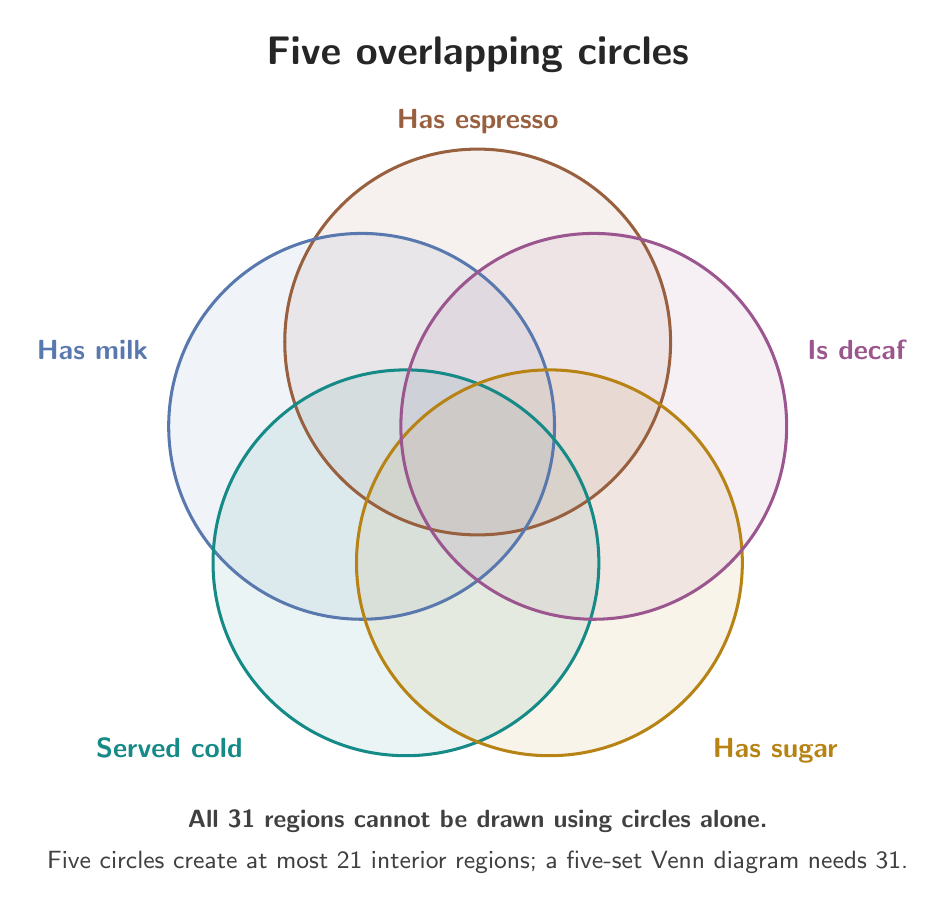
\begin{tikzpicture}[font=\sffamily, line width=1.1pt]
  % This is a maximal circle arrangement, not a five-set Venn diagram.
  % Five circles have at most 22 planar regions (21 inside their union).
  % A true five-set Venn diagram needs 32 planar regions, including outside.
  \node[font=\sffamily\bfseries\Large, text=black!85] at (0,5.2)
    {Five overlapping circles};
  \foreach \angle/\colour in
    {90/espresso,162/milk,234/cold,306/sugar,18/decaf}{
      \fill[\colour,fill opacity=0.09] (\angle:1.55) circle (2.45);
  }
  \foreach \angle/\colour in
    {90/espresso,162/milk,234/cold,306/sugar,18/decaf}{
      \draw[\colour] (\angle:1.55) circle (2.45);
  }
  \node[text=espresso,font=\sffamily\bfseries] at (0,4.35) {Has espresso};
  \node[text=milk,font=\sffamily\bfseries,anchor=east] at (-4.05,1.45) {Has milk};
  \node[text=cold,font=\sffamily\bfseries,anchor=north east] at (-2.85,-3.35) {Served cold};
  \node[text=sugar,font=\sffamily\bfseries,anchor=north west] at (2.85,-3.35) {Has sugar};
  \node[text=decaf,font=\sffamily\bfseries,anchor=west] at (4.05,1.45) {Is decaf};
  \node[align=center,text=black!75,font=\sffamily\small] at (0,-4.8)
    {\textbf{All 31 regions cannot be drawn using circles alone.}\\[4pt]
     Five circles create at most 21 interior regions; a five-set Venn diagram needs 31.};
\end{tikzpicture}
\end{document}
